\documentclass[aspectratio=1610,12pt]{beamer}
\usepackage{setspace}
\usepackage[utf8]{inputenc}
%\usepackage{hyperref}
\usepackage[spanish]{babel}
\usepackage{amsmath}
\usepackage{amssymb}
%\usepackage[procnames]{listings}
\usepackage{listings}
\usepackage{textcomp}
\usepackage{lmodern}
%\usepackage{enumitem}
\usepackage{enumerate}
%\usepackage{wrapfig}
%\usepackage{multirow}
\usepackage{tikz}
\usepackage{graphicx}
%\usepackage{soul}
%\usepackage[dvipsnames]{xcolor}
\usepackage{xcolor}
%\usepackage[table]{colortbl}
%\usepackage{applekeys}
%\usepackage[default]{opensans}
%\usepackage{lato} 

% fonts ----------------
\usepackage[T1]{fontenc}
%\usepackage[sfdefault]{AlegreyaSans}
% The 'sfdefault' option to make the base font sans serif
\renewcommand*\oldstylenums[1]{{\AlegreyaSansOsF #1}}
% fonts ----------------

% Background ------------------------------------
\usebackgroundtemplate{
	\tikz[overlay,remember picture] \node[opacity=0.02, at=(current page.center)] {
		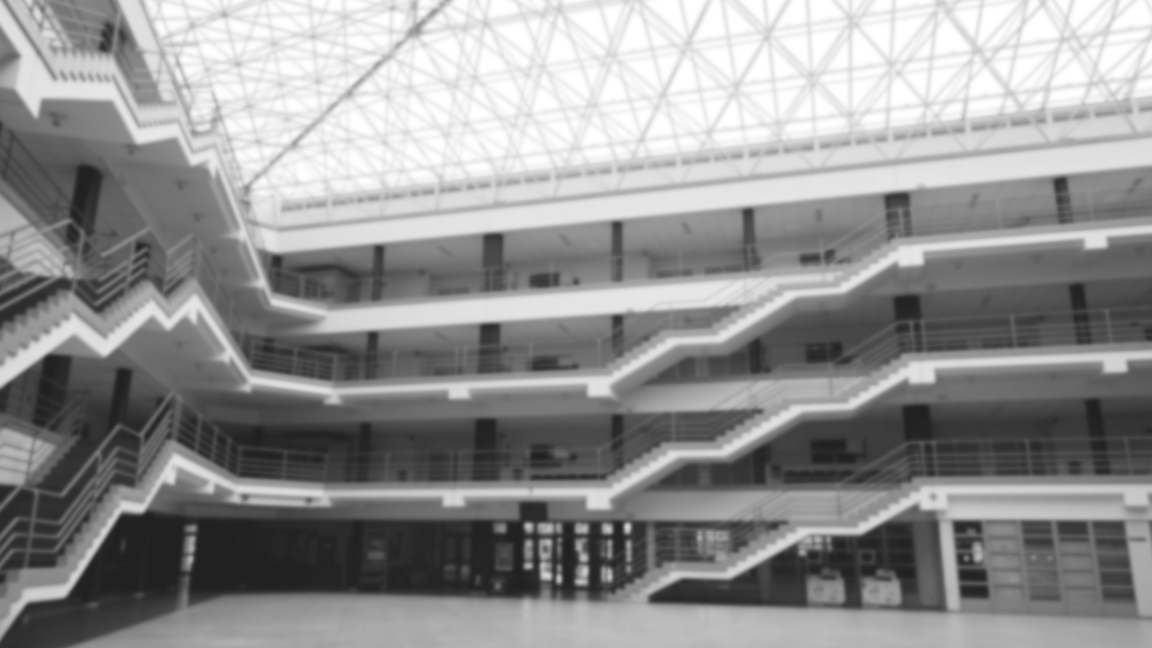
\includegraphics[height=\paperheight,width=\paperwidth]{../images/fondo_ucm}};
}
% Background ------------------------------------

% Theme choice:
\usetheme{CambridgeUS}
\usecolortheme{dove}

% Definiendo colores ----------------------------
\definecolor{pantoneblack}{RGB}{30,30,30}
\definecolor{pantone200}{RGB}{183,18,52}
\definecolor{pantone021}{RGB}{254,80,0} %naranja
\definecolor{oro}{RGB}{155,137,66}
\definecolor{plata}{RGB}{151,148,146}
\definecolor{rosa}{RGB}{253,233,235}
\definecolor{posit}{RGB}{254,249,231}
% colores listing
\definecolor{gray95}{gray}{.95}
\definecolor{keywords}{RGB}{255,0,90}
\definecolor{comments}{RGB}{0,0,113}
\definecolor{red}{RGB}{160,0,0}
\definecolor{green}{RGB}{0,150,0}
\definecolor{marino}{RGB}{18,10,143}
% colores beamer
\setbeamercolor{title}{fg=white!90!red,bg=pantone200!90}
\setbeamercolor{frametitle}{fg=pantone200!80!black}
\setbeamercolor{structure}{fg=oro}
\setbeamercolor{block title}{fg=white,bg=pantoneblack}
\setbeamercolor{alertblock title}{bg=pantoneblack}
\setbeamercolor{block title example}{bg=plata!50,fg=plata!140}
\setbeamercolor{block body example}{bg=plata!10}
\setbeamercolor{block title alerted}{bg=pantone200,fg=white}
\setbeamercolor{block body alerted}{bg=pantone200!10}
% Definiendo colores ----------------------------

% Fondo ------
% https://biblioteca.ucm.es/edicionweb/bancos-de-imagenes

% --------

% Comandos -------------
\providecommand{\consola}[1]{\texttt{\colorbox{pantoneblack}{\textcolor{white}{#1}}}}
\lstset{upquote=true}
% -----------------------

% Haz que las secciones tengan el mismo formato
\setbeamerfont{section title}{size=\LARGE, series=\bfseries}
%\setbeamercolor{section title}{fg=blue}
\setbeamertemplate{section page}{
	\begin{centering}
		\usebeamerfont{section title}
		\usebeamercolor[fg]{section title}
		\insertsection\par
	\end{centering}
}

\setbeamersize{text margin left=0.75cm, text margin right=0.75cm}

% Listing ---------------------------------------
\lstset{
	% Configuración de colores ---
	backgroundcolor=\color{gray95}, % Color de fondo suave
	basicstyle=\ttfamily\footnotesize,
	keywordstyle=\color{keywords}\bfseries, % Estilo de las palabras clave
	stringstyle=\ttfamily\color{green},%Color de las cadenas de texto
	commentstyle=\color{green}, % Color de los comentarios
	identifierstyle=\color{marino}, % Estilo identificadores de variables
	rulesepcolor=\color{pantoneblack},
	% Formato de números de línea ----------
	numbers=left, % none
	numberstyle=\scriptsize\color{gray}, % Estilo de los números de línea
	stepnumber=1, % Cada línea tiene número
	numbersep=10pt, % Separación de los números de línea
	%numberfirstline = false,
	% Características del código ---
	tabsize=2, % Tamaño de la tabulación
	showspaces=false, % No mostrar espacios
	showstringspaces=false, % No mostrar espacios en cadenas de texto
	showtabs=false, % No mostrar tabulaciones
	frame=single, % Poner un borde alrededor del código / Ltb - no ponerlo
	%framerule=0pt,
	breaklines=true, % Permitir que las líneas largas se dividan
	breakatwhitespace=true, % Dividir en espacios cuando sea posible
	captionpos=b, % Posición de la leyenda
	keepspaces=true, % Mantener espacios
	% Otros -----
	aboveskip=0.25cm,
	escapeinside={(*@}{@*)}, % Permitir comandos LaTeX en el código
	morekeywords={*,...} % Añadir palabras clave si es necesario
%	framextopmargin=2pt,
%	framexbottommargin=2pt,
%	framexleftmargin=0cm,
%	framesep=0pt,
%	rulesep=.4pt,
}
\setbeamertemplate{navigation symbols}{
	\insertslidenavigationsymbol
	%\insertframenavigationsymbol
	%\insertsubsectionnavigationsymbol
	%\insertsectionnavigationsymbol
	%\insertdocnavigationsymbol
	%\insertbackfindforwardnavigationsymbol
}
\addtobeamertemplate{navigation symbols}{}{%
	\usebeamerfont{footline}%
	\usebeamercolor[red]{footline}%
	\hspace{2em}%
	\insertframenumber %/\inserttotalframenumber
}
%\setlength{\parindent}{0pt} %Quitar sangrado primera linea
%\lstdefinestyle{consola}
%{basicstyle=\footnotesize, backgroundcolor=\color{gray75}} %\scriptsize\bf\ttfamily
%\lstdefinestyle{Python}
%{language=Python}
\providecommand{\consola}[1]{\footnotesize\normalsize\texttt{\colorbox{negro_w}{\textcolor{white}{#1}}}}

% Title page details: 
%\subtitle{(Apuntes de repaso)}
\author[Francisco Gárate]{Francisco Gárate Santiago - fgarate@ucm.es}
\institute{UCM}
\date{Master en Ciencias Actuariales y Financieras (2024-2025)}
%\logo{
\includegraphics[scale=0.2]{/home/paco/Dropbox/CURSOS/IFRS17/images/Logo.png}}
\logo{
\includegraphics[scale=0.2]{../images/Logo.png}}
